%!TeX root = main.tex
\documentclass[main.tex]{subfiles}

\begin{document}

\chapter{Database approach}
\vspace*{-1\baselineskip}

\section{Screening studies}

Research on the adsorption properties of zeolites in particular, and nanoporous materials in general, aims at understanding the nature and respective importance of the different interactions that drive the adsorption phenomenon. Afterwards, this understanding can be turned into principles, which are then applied to predict the adsorption capacities of similar materials on similar gases, where these principles remain valid.

The natural starting point for this research is a study of a particular material with a particular gas, which leads to particular observations that may then be generalized. Many such studies have been performed and published on zeolites, each involving a considerable amount of work, which provide very precise results on a given topology, with up to a few \SiAl ratios. Yet, the conclusions can seldom be carried over to provide predictions on other topologies.

The converse strategy consists in doing screening studies, in which a vast array of structures is tackled at the same time. Given the cost of doing so experimentally, these studies are mostly computational, thus providing less precise results than actual experiments, but on a broader scale.

Most zeolite screening studies focus on all-silica zeolites, an approach that sidesteps the issue of placing cations. However, most zeolite adsorption applications require cationic zeolites, since cations critically increase the adsorption capacity of the materials.

Even among the few studies which tackle cationic zeolites across topologies and \SiAl ratios, not all properly place cations in the framework, although it is known that this can lead to incorrect subsequent adsorption measurements [REF]. For example, [10.1021/acs.langmuir.2c03089] targets 57 different topologies with 5 different possible cations, but fails to mention where these are placed before the start of the GCMC simulations, likely resulting in them being trapped in a non-optimal placement. [10.1038/NMAT3336] also screens cationic zeolites, but places cations at the so-called ``minimum energy positions'' instead of using a robust method like parallel tempering; they also use a force field made for FAU zeolites only, which is inadequate to screen other zeolites. 
We are only aware of the works of Sholl [REF], which tackles many zeolite with various \SiAl ratios for screening purposes, that properly places cations through parallel tempering.

In this chapter, we explain how we constitute a database of cationic zeolite structures and how it can be used for isotherm prediction.

\section{Adsorption isotherm}

\subsection{Definition and classification}

\begin{figure}[b]
	\centering
	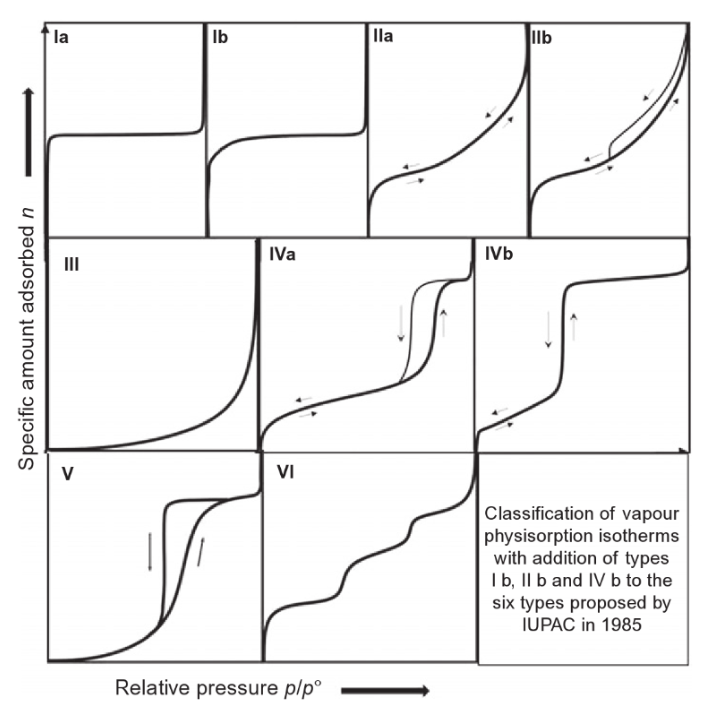
\includegraphics[width=0.6\columnwidth]{figures/database/IsothermTypes.png}
	\caption{Classification of gas isotherm by IUPAC, taken from \cite{Rouquerol2013}, adapted from \cite{IUPAC1985}. $p^0$ designates the saturation pressure of the adsorbate.}\label{fig:IUPACisotherms}
\end{figure}

The behaviour of a materials with respect to the adsorption of a gas is typically assessed by measuring the evolution of its adsorption capacity with pressure, at a fixed temperature. The resulting curve is called an isotherm, and it is usually classified according to its general shape into one of several possible categories, represented on \cref{fig:IUPACisotherms}.

The shape of the isotherm depends on the surface of the materials, the strength of its interaction of the adsorbate and of the adsorbate-adsorbate interactions. For example, type I isotherms are typical of materials with very small external surface and monodisperse pores of small size, where adsorption quickly reaches saturation. On the other hand, type III isotherms occur when the adsorbent-adsorbate interaction is weak and adsorption is not limited by the pore size (either because adsorption occurs on the external surface or because the pores are very large). Some of these types exhibit hysteresis loops: for example, type IV(a) isotherms, typical of mesoporous adsorbents, have the adsorption branch lower than the desorption branch (when the gas is withdrawn), which comes from the capillary condensation of the adsorbate at high pressure. Real isotherms are often combinations or slight variations of these idealized types. [10.1007/s10450-016-9766-0]

At very low pressure, all isotherms are expected to be linear: this is Henry's law, and Henry's adsorption constant $K$ is proportional to the slope of the isotherm. In that limit, all adsorbates behave like ideal gases since, by definition, there is no adsorbate-adsorbate interaction at low enough pressure.

The other end of the pressure spectrum is more complex. When adsorption occurs on the external surface of the adsorbent, for instance with clays, and if adsorbent-adsorbent interactions are strong enough to allow multi-layer adsorption, then the number of adsorbed species never stops growing with increasing pressures. However, with zeolites and more generally any adsorbent where adsorption occurs in finite pores, the adsorption capacity plateaus at high pressure when all the pores are filled with the adsorbate. It should be mentioned though that the adsorption capacity can still increase beyond that limit, because of the compressibility of the adsorbate in liquid or supercritical state. These regimes of extremely high pressure (beyond $\qty{100}{MPa}$) are of lesser industrial relevance because reaching these conditions is costly and hazardous. [REF]

\subsection{Experimental observation and numerical prediction}

Experimentally, adsorption isotherms are drawn by progressively increasing the input pressure of the adsorbate in the material at the fixed temperature, and measuring the amount adsorbed. The desorption isotherm follows up by progressively decreasing the input pressure, and similarly measuring the amount of adsorbate.

The measurement itself usually consists in either of the three following methods:
\begin{itemize}
	\item volumetry: a fixed amount of gas at the target pressure is put in contact with the adsorbent, and what is measured is the difference of pressure before and after adsorption.
	\item breakthrough: the gas starts flowing through the adsorbent at a given time, and the outlet concentration and volumetric flowrates are measured.
	\item gravimetry: the difference in mass of the sample containing the adsorbent before and after adsorption is measured by balancing its weight against buoyancy.
\end{itemize}
By reproducing the experiment with a reference gas (usually \ce{N_2} or \ce{Ar}), these techniques give access to the net adsorption, which is the absolute amount of adsorbed species minus that which would be in a fluid occupying the same space as the adsorbent at the same pressure and temperature. Knowledge of the volume of adsorbent allows retrieving the absolute adsorption capacity, which is directly accessible in simulations.

Some more anecdotic isotherm measurement techniques including impedance spectroscopy [REF] as well as NMR [REF] allow obtaining directly the absolute adsorption, but these methods are much too costly to be used routinely.

The adsorption capacity can be predicted numerically through Grand Canonical Monte-Carlo (GCMC) simulations, as explained in \cref{GCMC}. Beyond the limits due to the precision of the energy computation, either from a force field or from DFT, and convergence of the simulations, those are also dependent on a model of the adsorbent which cannot take into account the complexity of real materials. In the case of zeolites, the location of the aluminium and of the cations has already been discussed through \cref{cationzeolites}, but more generally, all kinds of defects and small crystal size effects can lead to experimental isotherms differing from the simulated counterparts. This limits the accuracy of individual numerical simulation compared to precise experimental adsorbents, but they remain useful to extract tendencies and direct the search for new adsorbents, which will be experimentally tested eventually.

\section{Database constitution}

Finding general tendencies in the adsorption behaviour across zeolites requires doing the analysis of many different structures. To do so, the first step consists in establishing a database of models for the materials themselves. The general simulation workflow, starting from the idealized zeolite structure defined by its topology, down to the cation placement, has already been described in \cref{cationzeolites}. To summarize, the two steps are:
\begin{enumerate}
	\item Aluminium placement. Start by finding the minimum \SiAl ratio by replacing as many silicium with aluminium atoms as possible, with random exchanges and restarts. Check multiple supercell sizes. Then, starting from these filled structures, replace some aluminium by silicium atoms at random and do more exchange steps to generate 6 aluminium placements for each target \SiAl ratio.
	\item Cation placement, using either parallel tempering or shooting star simulations. The only cation used is sodium.
\end{enumerate}

\subsection{Aluminium placement}

The current database contains 6 aluminium placements for all 239 known and not interrupted zeolite topologies, with \SiAl ratios of \num1, \num{1.23}, \num{1.4}, \num{1.7}, \num{2}, \num{3}, \num{5} and \num{10}. The actual \SiAl ratios of each structures are those closest to the previous references, which may sometimes differ. When the minimum \SiAl ratio (presented in \cref{table:zeosial}) is not among the previous references, it is added separately, and the lower \SiAl ratios cannot be generated. For example, the list of actual \SiAl ratios for topology YUG is $1.56$, $\frac{121}{71}\approx1.704$, $2$, $3$, $5$ and $\frac{349}{35}\approx9.971$.

The algorithm sometimes fails at finding 6 distinct aluminium placements: in that case, the maximum number of distinct placements is kept. To check whether a new placement is distinct from previous ones, the following algorithm is used. First, for each topology, the list of T-sites is mapped to the list of integers between $1$ and $N$, the number of T-sites of the topology. Each placement is represented by a sequence of $N$ bits, where a bit of 1 at position $i$ indicates an aluminium in T-site $i$ and 0 stands for silicium. Then, all $M$ symmetries of the topology are applied to the placement: this results in $M$ $N$-bit sequences. The (lexicographically) smallest among those serves as a unique signature that identifies the aluminium placement. Then, when a new placement is found, is signature is computed as previously and compared to those already encountered: if it is different from all of them, the new placement is stored.

In the case where $\SiAl = 1$ for example, there can be up to only 2 distinct aluminium placements that obeys L\"owenstein's rule: taking an arbitrary T-atom as a reference, one placement corresponds to that reference set to Al, and the other to that reference set to Si. For many topologies, these two placements are actually symmetry-equivalent, so they share the same signature and only one of them is actually stored. This is not necessarily the case however: for example, topology JSW has two distinct aluminium placements for $\SiAl = 1$.

Overall, \num{8983} different structures with aluminium placed were generated.

\subsection{Cation placement}

For all 239 known and non-interrupted topologies, and for each of the up to 6 different aluminium placements corresponding to the minimum \SiAl, a shooting star simulation was launched with the hot run at \qty{2000}K for \num{20000} cycles (and \num{2000} initialization cycles), spawning one cold simulation every \num{100} cycles. Each of the resulting \num{200} cold simulations run at \qty{300}K for \num{10000} cycles. This served as an experiment to assess the convergence of the simulations: out of the 239 topologies, 57 converged in less than \num{5000} cycles (averaged across aluminium placements). For these topologies, shooting star simulations were run for all previously created aluminium placements across the different \SiAl ratios, using the same parameters (except for the number of cold cycles raised to \num{15000}). For shooting star simulation, the \num{200} cold simulations are divided into six groups, and for each of these groups, the structure with the lowest corresponding energy is kept. Hence, this methodology yields 6 cation placement per structure.

% TODO: discuss and choose whether lowest energy is better than random.

Overall, \num{14268} different structures with both aluminium and cations placed were obtained.
% TODO: update this number


\section{Prediction}

\subsection{Isotherm fitting}

\subsection{Simple models}

\subsection{Machine learning}

% topology

\subsection{Perspectives}

% Other zeolite materials



\end{document}
